
%%%%%%%%% MASTER -- compiles the sections

\documentclass[11pt,letterpaper]{article}
\setlength{\parskip}{1ex plus 0.5ex minus 0.2ex}

\usepackage{graphicx}
\usepackage{hyperref}
\hypersetup{
    colorlinks,%
    citecolor=black,%
    filecolor=black,%
    linkcolor=black,%
    urlcolor=black
}
\usepackage{listings} %for source code figures
\usepackage[toc,xindy,style=long3colheaderborder,footnote]{glossaries}
%\usepackage[toc,xindy]{glossaries}
\makeindex
\makeglossaries


\newglossaryentry{speedup}{name={speedup}, description={The overall time gain of a process or computation.}}

\newglossaryentry{time complexity}{name={time complexity}, description={The time it takes for a process to run.}}


\newglossaryentry{paralellization}{name={paralellization}, description={Taking independent or semi-independent processes, and processing them in parallel (at the same time).}}

\newglossaryentry{granularity}{name={granularity}, description={The time or portion of the process that each iteration / sub-process takes.}}

\newglossaryentry{HPC}{name={HPC}, description={High Performance Computing.}}


%%%%%%%%%%%%%%%%%%%%%%%%%%%%%%%%%%%%%%%%%%%%%%%%%%%%%%%%%%%%%%%%%%%%%%%%%
\pagestyle{plain}                                                      %%
%%%%%%%%%% EXACT 1in MARGINS %%%%%%%                                   %%
\setlength{\textwidth}{6.5in}     %%                                   %%
\setlength{\oddsidemargin}{0in}   %% (It is recommended that you       %%
\setlength{\evensidemargin}{0in}  %%  not change these parameters,     %%
\setlength{\textheight}{8.5in}    %%  at the risk of having your       %%
\setlength{\topmargin}{0in}       %%  proposal dismissed on the basis  %%
\setlength{\headheight}{0in}      %%  of incorrect formatting!!!)      %%
\setlength{\headsep}{0in}         %%                                   %%
\setlength{\footskip}{.5in}       %%                                   %%
%%%%%%%%%%%%%%%%%%%%%%%%%%%%%%%%%%%%                                   %%
\newcommand{\required}[1]{\section*{\hfil #1\hfil}}                    %%
\renewcommand{\refname}{\hfil References Cited\hfil}                   %%
\bibliographystyle{plain}                                              %%
%%%%%%%%%%%%%%%%%%%%%%%%%%%%%%%%%%%%%%%%%%%%%%%%%%%%%%%%%%%%%%%%%%%%%%%%%

%PUT YOUR MACROS HERE

\date{April 29th, 2011}
\title{High Performance Computing \\
	in the University of Idaho \\
	College of Natural Resources}

\author{Colby Blair \\
	Computer Science Undergraduate \\
	University of Idaho Computer Science Department
}


\begin{document}

\section*{Letter of Transmittal}
\textbf{Subject.} High Performance Computing in Natural Resources.

\textbf{Purpose.} This report focuses on the programming challenge faced in computing current research. The goal is to introduce the concept of High Performance Computing (HPC) to an audience that may understand mathematics and habitat data, but doesn't have a lot of training with programming. This report covers the concept of Parallel Computing, and the motivation to do so. It then demonstrates implementation of Parallel Computing on a High Performance Computing Cluster (HPCC). It then talks about real algorithms in current research, and their parallel equivalents on several University of Idaho HPC Clusters. It then shows the results  of using an HPCC and Parallel programming, to motivate others in CNR to embrace HPC in their research projects.

\textbf{Background.} A large part of animal studies in CNR is tracking animal movement. As an animal moves through a landscape over time, its recorded locations can create probabilities of where that animal may be at any one time. One method of probability mapping uses the Brownian Bridge model (Horne, Garton, Krone, and Lewis et al 2007). The Brownian Bridge alone, however, doesn't tell us anything about the habitat. The Synoptic model of Space Use (Horne, Garton, and Rachlow et al 2007) provides us with habitat data based off of animal locations. Combining the Brownian Bridge model with the Synoptic Model allows us to more intelligently select habitat data that affects animal movement. But it is also very computationally expensive.

\textbf{Preliminary Work}. The graduate student leading the project has already earned his Masters on this study. He then went on to pursue his Ph.D., and the author joined the project around February of 2010. Our first challenge was to create a parallel implementation of the Brownian Bridge model. This shortened the computer process time of 1 goat from 144 hours to under 1 minute. But it was quickly realized that Brownian Bridge was not enough; we needed Synoptic Modeling. Merging the two methods is what we are finishing now.

\thispagestyle{empty}

\pagebreak

\maketitle

\thispagestyle{empty}

\pagebreak

\thispagestyle{empty}
\tableofcontents
\listoffigures

\pagebreak

\begin{abstract}
With today's exponential increase of data, the demand for processing is outpacing the supply. The way we 
processed data yesterday would take years to do today. Unfortunately, the lake of fluency with computing in
today's research proposals results in processing a fraction of the data collected. This weakens research 
projects, and leads to a lot of unnecessary data collection. 

Today's researchers must become fluent with the language of High Performance Computing. Not only can
HPC strengthen the results of research projects, but it can also be overused. With an understanding of the 
rules of HPC, embarassingl parallel gains in processing will occur. The gains and pitfalls can suprise even
the experienced programmer, but the concepts of HPC are simple, and the benefits are great.

\end{abstract}

\setcounter{page}{1}

\pagebreak


%%%%%%%%% SUMMARY -- 1 page, third person
% e.g:  "The PI will prove" not "I will prove"

%Introduction / Summary (1 page).  The following information is typically included in proposal introductions for this 
%grant. The summary should lead to the proposal body but it should also be a self-contained document, 
%summarizing what is being proposed and why.   
 
% Provide appropriate background that sets the context for the problem and the objectives. 
%State the specific problem (may also be thought of as a need, central research question, or hypothesis) 
%your research will address. 
% State the objectives of the proposed research. 
%State any limits of the proposed research  (may not be needed). 
%Summarize the research methods you will use to achieve research objectives (if clearly covered elsewhere 
%in the introduction, a separate section may not be needed). 


%\required{Project Summary}
\section{Project Summary}
% This should be a brief statement of the problem you plan to address.
% It should look something like an abstract. 

\subsection{Background}

In the areas of ecology and bioinformatics, there is an explosion of data. The
amount of bioinformatics data in research institutions doubles every 9 months 
\cite{james}. Gains in processing power, however, are decreasing, as the end
of Moore's Law's approaches \cite{gordon_moore}. As processor speed gains decrease, 
a vacuum for high performance computing is growing. More and more data has 
to be ignored. Data that was expensive to collect.

In spite of the growth of data and platue of processor computing power, a 
solution exists that allows scientists and mathematicians to conduct their 
research. High Performance Computing (HPC) networks groups of computers 
together as one supercomputer. HPC then uses parallel programs that do many 
of their tasks in parallel, or at the same time. This reduces run time. 
The result is a resource that allows researchers to do years worth of 
processing in months.

\subsection{Problem Statement}

Unfortunately, computing is typically an afterthought in most research projects.
Most researchers focus on data collection, and assume that the power to
process their data is cheap and widely available. This assumption leads to 
overcollection of data, and almost no relative analysis of that data. Without
consultation of computer scientists, most scientists' research is a fraction of
what it should be.

\subsection{Objectives}

The proposal here is to conduct research on existing algorithms used in 
CNR, and to parallelize them on a HPC cluster. Algorithms will be take from 
recently completed and ongoing research projects, and they will be demonstrated
in an HPC environment. Concepts of HPC and Parallel Programming will be covered,
and their implementation in current research will be shown.

Demonstrating HPC and Parallel Programming methods in research could be very 
beneficial to fellow researchers. It will create interest in computer science,
and encourage a much needed interdisciplinary dialogue. More project proposals 
would include more realistic processing projections. Less research data would be
thrown away, and overall projects' success would rise.

The objective of this project proposal is to establish a computing cornerstone
in the College of Natural Resources. It is to educate scientists and 
mathematicians with HPC concepts. The objective is to spread experience with 
computing on a big scale, so that scientists can shape their research around
what is achievalbe. The objective will also affect how mathematicians develop 
their algorithms.

Limitations to the project are drawn at the operating system level. Some detail
is given on the HPC Operating System, but building one is beyond the scope of 
the research. Operating systems will only be discussed as much as is needed
to allow readers to work the software. The rest of the operating system 
documentation should be enough.

%\required{Intellectual Merit}
% This is why your project is interesting and will help further
% knowledge in the field of mathematics. 

%\required{Broader Impacts}
% There are 4 kinds of broader impacts.
% 1. advance discovery and understanding while promoting teaching,
% training and learning
% 2. broaden the participation of underrepresented groups
% 3. disseminated broadly to enhance scientific and technological
% understanding
% 4. benefits of the proposed activity to society


\section{Parallel Concepts}
\label{sec:par_con}
The concept of parallel computing is simple, despite the complex impression many get at first glance.
Parallel computing equates to many real life situations, in which a lot of work needs to be done by a lot of 
resources, in the quickest time possible. The bottom line in both is to keep as many of those resources busy
at one time as possible.

\subsection{Parallel Bingo}
\label{sec:bingo}
Let's consider a real world example. A group of a hundred mathematicians meet one night to play a game of 
bingo. Curious as mathematicians are, they realize that there are a finite amount of bingo boards. The group
then asks; for each sequence of numbers called, which boards are the best? Out of a certain amount of 
number sequences, which boards win the most?

The mathematicians start their experiement. A sequence of numbers is pre-recorded, and then one 
mathematician begins checking each board to see how many each each needs to get a win. But the other 
nintety-nine mathematicians begin to realize that only one doing all the work will take a while, and they might
as well help.

Each mathematician gets in line. At the front of the line, a unique bingo board is handed out, along with a 
paper with the number sequence for the current game. For each game, all the papers have the same number 
sequence. Each mathematician goes back to their table and begins marking the bingo board. When a bingo is
reached, the mathematician writes how many numbers in the sequence the board needed for the win. Lower is
better, of course. They then go to the back of the line, and will report their results when their turn comes again.

\begin{figure}[h]
	\begin{center}
		\includegraphics[width=50mm]{images/bingo.png}
		\caption{Mathematicians getting bingo boards, and returning to the end of the line with results} 
		\label{bingo}
	\end{center}
\end{figure}

\subsection{Speedup Introduction}
The biggest question in parallel computing or processes is, of course, how much faster is it? Formally, what is the \gls{speedup}? 
In Section \ref{sec:bingo}, for example, we would expect one hundred mathematicians to do the work of one 
mathematician in $1/100$th of the time. But reviewing Section \ref{sec:bingo}, is this actually the case? No,
in fact. Each of the one hundred mathematicians spent considerable time in line. Since one mathematician
doing all the work would have never spent time in line, the line time counts against any speedup the group
has otherwise. This leads to our first formal point with Amdahl's Law:

\begin{figure}[h]
	\begin{center}
		\LARGE
		\begin{tabular}{l r}
			$ A $		&	$ = \frac{1}{(1 - P) + \frac{P}{N}} $ \\
		\end{tabular}

		\normalsize
		\begin{tabular}{l l}
			$ where $  & \\
					&	$ P $ is the portion of the program that can be 'parallelized' \\
					&	$ N $ processors or workers \\
					&	$ (1 - P) $ is the sequential / serial portion (cannot be parallelized) \\
		\end{tabular}
		\caption{Amdah's Law. \cite{amdahl}} 
		\label{amdahl}
	\end{center}
\end{figure}
\normalsize

$ P $ informally is the portion of the program that can be split up into sections, each of which can be worked 
on simultaniously. The name for this process is \gls{paralellization}. Informally, Ahmdahl's Law shows that 
the higher $ P $, or portion of work that can be split up, the more beneficial adding more workers ($ N $) is. Too many workers, and the benefit decreases.

In the Section \ref{sec:bingo}, this makes sense. There is not much benefit committing too many more
mathematicians than bingo boards. The time spent processing bingo boards still improves, but the gain
shrinks compared to the constant time of totaling all the boards together. Amdahl's Law highlights the 
relationship between parallel work and workers, and we can see this relationship more formally graphed:

\begin{figure}[h]
	\begin{center}
		\includegraphics[width=80mm]{images/amdahl_graph01}
		\includegraphics[width=80mm]{images/amdahl_graph02}
		\caption{Speedup comparisons,} 
		\label{amdahl_graph}
	\end{center}
\end{figure}

Figure \ref{amdahl_graph} compares speedups of the theoretical bingo game. The graphs highlight two points
from Amdahl's Law; larger gains with larger $ P $ values, and the law of diminishing returns. The right graph
shows the benefits of parallelization when the time to process a bingo board is double what the left graph is.
As N approaches infinity, $ \frac{P}{N} $ approaches 0, so $ A $ approaches $\frac{1}{(1 - P)} $. 

In the bingo example, there may not be much to gain from this knowledge. But in more complicated problems,
this highlights one of the key goals of parallelization: decreasing $ (1 - P) $ and increasing $ P $. Informally,
taking as many of the processes out of the serial / sequential portion of the process, and getting them into
the parallel portion of the program. There are right and wrong ways of doing this, which this report will cover.
Processes or algorithms that already have high $ P $ values are 'embarrasingly parallel'.

\subsubsection{Maximizing P}
In Section \ref{sec:bingo}, serial time ( $ (1 - P) $ ) and parallelizable time ( $ P $ ) were accounted for. But 
overhead time was ignored. In the bingo example, this equals the time spent waiting in line. As more 
mathematicians ( $ N $ ) are added, overhead increases. Since waiting in line is not parallelizable, this adds 
to the serial time ( $ (1 - P) $ ). This is as true in theory as it is in real computing systems. The resulting 
equation is:

\begin{figure}[h]
	\begin{center}
		\LARGE
		\begin{tabular}{l r}
			$ A $		&	$ = \frac{1}{((1 - P) + (T_P * N)) + \frac{P}{N}} $ \\
		\end{tabular}

		\normalsize
		\begin{tabular}{l l}
			$ where $  & \\
					&	$ P $ is the portion of the program that can be 'parallelized' \\
					&	$ N $ processors or workers \\
					&	$ (1 - P) $ is the sequential / serial portion (cannot be parallelized) \\
					&	$ (T_P * N) $ is the overhead \\
		\end{tabular}
		\caption{Amdah's Law (Figure \ref{amdahl}) with Overhead. } 
		\label{amdahl_overhead}
	\end{center}
\end{figure}
\normalsize

This adds complexity to Amdahl's Law, but adds logical results to calculating speedups:

\begin{figure}[h]
	\begin{center}
		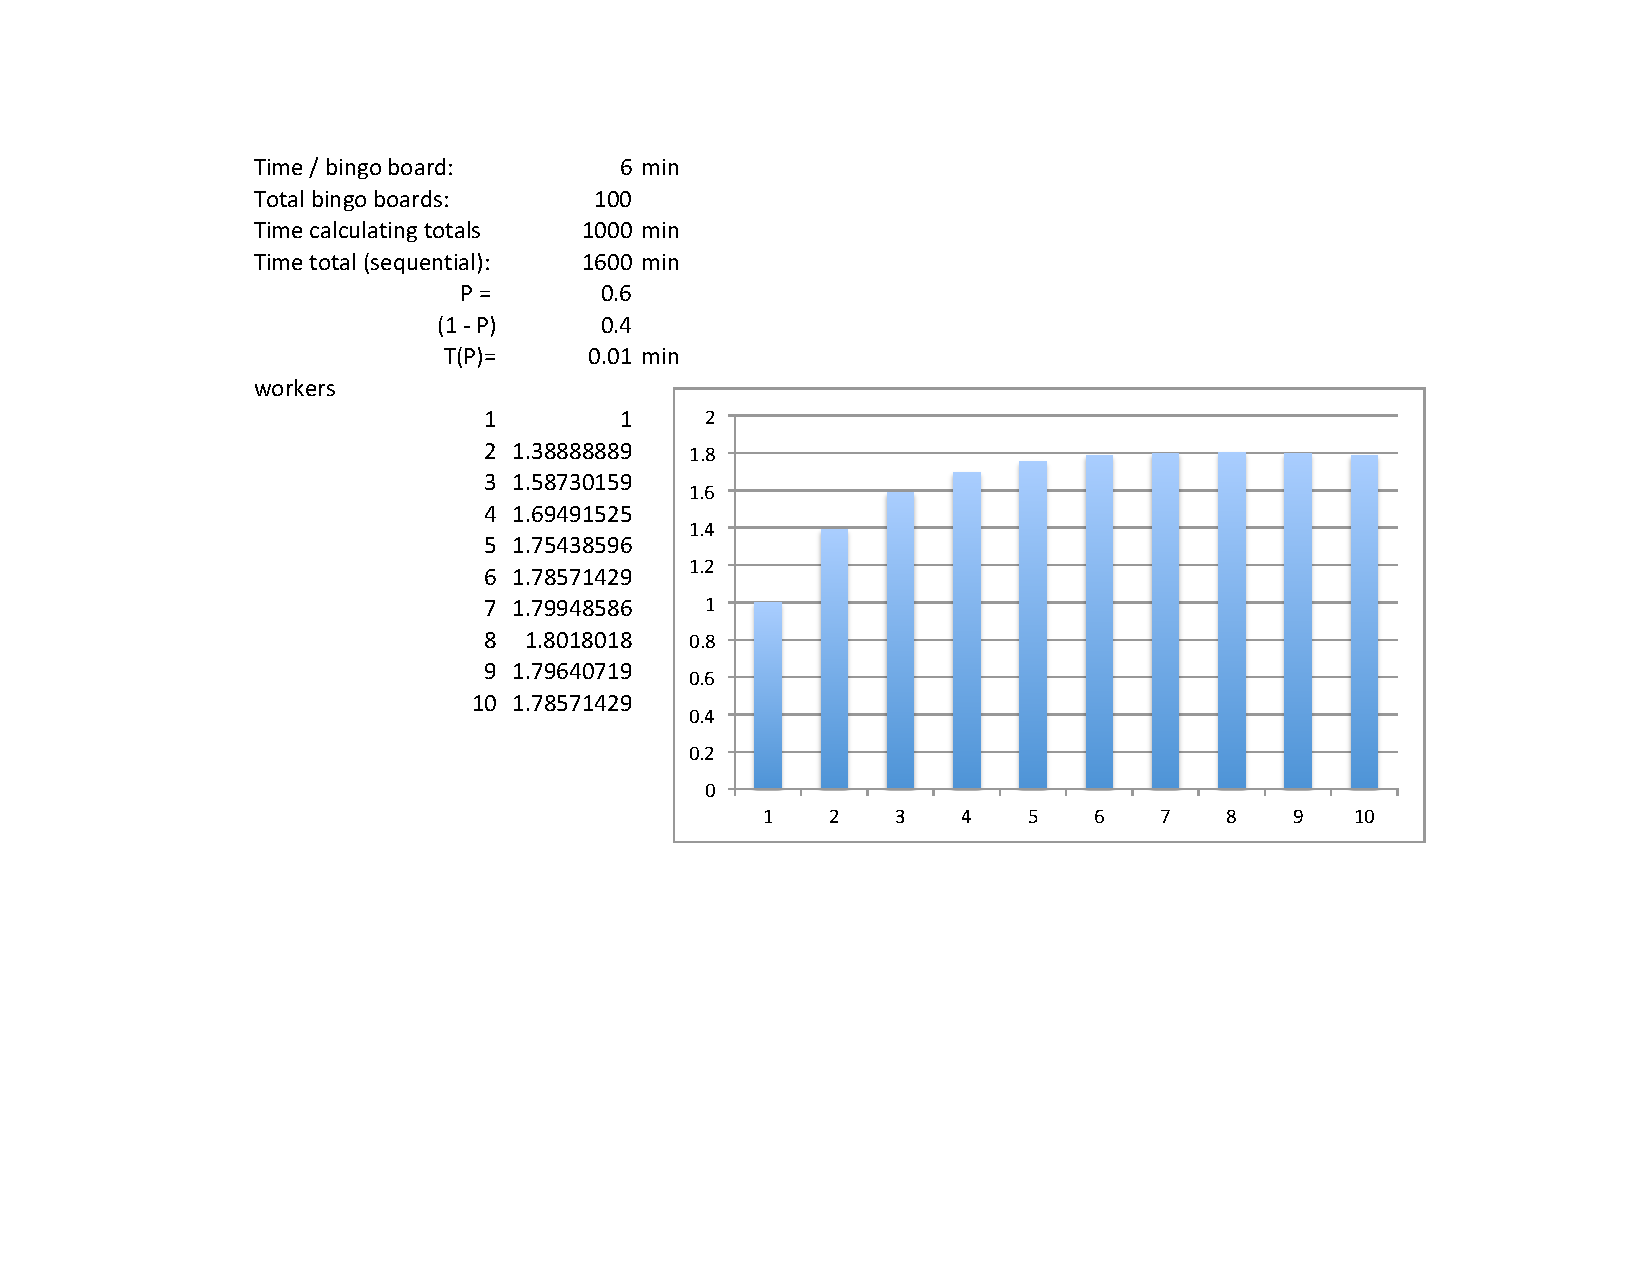
\includegraphics[width=130mm]{images/amdahl_overhead}
		\caption{Speedup comparisons including overhead} 
		\label{amdahl_overhead_graph}
	\end{center}
\end{figure}

Figure \ref{amdahl_overhead_graph} shows that not only the law of diminishing returns, but a negative 
benefit. Adding more workers actual slows parallel processes down at a certain point. In the bingo example,
at a certain point, adding more workers just creates longer lines and doesn't actually speed bingo board 
checking up. For many algorithms, $ P $ can only be a fairly small size. The best value for $ N $ will then only be 1. If $ P $ is not very big to begin with, than any $ N $ greater than 1 will cause a slowdown instead 
of speedup. Thus, even though some programs can be parallelized, if $ N > 1 $ causes a slowdown, they 
shouldn't.


\subsection{Speedup Summary}
Figure \ref{amdahl_overhead_graph} highlights two other key goals of parallelization: minimize $ T_P $, and 
maximize \gls{granularity} \cite{mit}. Granularity is how much work time each iteration or sub-process takes. 
In maximizing \gls{granularity}, $ P $ is maximized. In the bingo example, this means taking any process the 
totaller has to do at the end, and seeing if each mathematician can do it for their respective bingo board. This
saves the totaller time at the end, decreases serial time ( $ (1 - P) $ ), and increases parallel time ( $ P $ ).

The correct way to maximize $ P $ is to replace serial time processes with parallel time processes. The 
incorrect was is to simply inflate $ P $. If a process is not being moved from serial to parallel time, a bigger
$ P $ value will not lead to a real speedup. Informally, making more busy work for all the workers that doesn't
help reach the overall goal doesn't justify adding more workers. This may seem obvious, but is often 
attempted when $ N > 1 $ causes slowdowns. 

The analogy is that it is better to run optimized serial processes than it is to parallelize garbage. The former is
usually quicker anyway, and doesn't require more resources. This seems obvious, but the latter is often 
tried when parallelization is misinterpretted as a sledgehammer for making processes run faster.

\section{Parallel Programming}
Parallel programming is merely the application of parallel concepts. In Section \ref{sec:par_con}, the general
approach was discussed on how to recognize potentially parallelizable situations. Moving into parallel
programing, parallelization must be formalized a little more.

In Section \ref{sec:par_con}, tasks that happened over and over again were what were used to show the 
parallelization process. These repeated tasks are what are called iteration in computer science, and they are
one of the easiest speedup that can be gained in parallelization. Although there are other gains to be had,
this report will focus on iteration. 

\subsection{Data parallelism}
Data Parallelism is very similar to Task Parallelism. The difference practically is that instead of using libraries
in say R to parallelize tasks, we would just run the whole program parallel:
\scriptsize
\begin{lstlisting}
> R CMD BATCH primes.r -y 5 &
[1] 1228
> R CMD BATCH primes.r -y 7 &
[1] 1229
\end{lstlisting}
\normalsize

Above, we use the '\&' symbol in linux to run the process in the background. If our computer has multiple 
CPUs, the operating system will send each program to a free CPU. There is no need to profile the program
or calculate speedup. The speedup will always be ideal on independent data. Since it is so simple, it is 
encouraged as a first step towards parallelism. It does not, however, speed up each individual program run. 
If the program itself needs speedup, you need Task Parallelism.

These processes will die, however, when the user logs out. This becomes problematic when processes take a 
lot of time. A need for batch servers and schedulers grows, which are common in \gls{HPC} environments. 
These are discussed in Section \ref{sec:hpc}.

\subsection{Task parallelism}
Task Parallelism is when many tasks or processes are ran at one time. This is very similar to Data Parallelism,
in that Task Parallelism usually involves starting with some data and performing an operation on it. The
difference is that Task Parallelism ends up performing a slighlty different task on different data, where
Data Parallelism is the exact same task performed for many sets of data.

In your research project, parallel alarm bells should sound if you have an algorithm like the following:
\begin{figure}[h]
	\begin{center}
		\LARGE
		\begin{tabular}{l r}
			$ x $		&	$ = \sum_{i = 1}^1 f(i)$ \\
		\end{tabular}

		\normalsize
		\begin{tabular}{l l}
			$ where $  & \\
					&	$ f(i) $ is some function that uses $i$ \\
		\end{tabular}
		\caption{A potentially parallelizable algorithm} 
		\label{sigma}
	\end{center}
\end{figure}
\normalsize

For the layman, this means any function that is applied to many different values, and all the results can then
be collected. An example would be calculating how many numbers are prime upto a variable $ y $. The 
function would then be $ f(i) = 1 $ if $i$ is prime, $f(i) = 0$ if $i$ is not prime. So for 7, the equation is as
follows:

\begin{figure}[h]
	\begin{center}
		%\LARGE
		\begin{tabular}{l l}
			$ x $		&	$ = \sum_{i = 1}^1 f(i)$ \\
					&	$ = f(1) + f(2) + f(3) + f(4) + f(5) + f(6) + f(7)$ \\
					&	$ = 1 + 1 + 1 + 0 + 1 + 0 + 1 $\\
					&	$ = 5 $ \\
		\end{tabular}

		\normalsize
		\begin{tabular}{l l}
			$ where $  & \\
					&	$ f(i) = 1$ if $i$ is prime \\
					&	$ f(i) = 1$ if $i$ is not prime \\
		\end{tabular}
		\caption{How many primes factors are in a number} 
		\label{primes}
	\end{center}
\end{figure}
\normalsize

This may be a trivial example, but as numbers get bigger, it will take more time. The time requirements come
down to how you determine if a number is prime or not. This process can take a long time with big numbers.
Cryptography algorithms depend on it! Each $f(i)$ can be treated like the mathematicians and bingo boards
in Section \ref{sec:par_con}, so this algorithm has potential to be parallelized.

Using the R language, we can code Figure \ref{primes} as follows:
\scriptsize
\begin{lstlisting}
> 
> is.prime <- function(i) {
+ 	... #some R magic
+ }
> 
> y = 7
> sum = 0
> for(i in 1:y) {
+ 	sum <- sum + is.prime(i)
+ }
> 
> print(sum)
[1] 5
\end{lstlisting}
\normalsize

This is not the best way in R to write this, but is easier to understand. A method that better prepares us for
parallelism is using lapply:

\scriptsize
\begin{lstlisting}
> y <- 7
> sum <- 0
> results <- lapply(1:y, is.prime)
> for(i in 1:length(results)) {
+ 	sum <- sum + results[[i]][1]
+ }
> print(sum)
[1] 5
\end{lstlisting}
\normalsize

What if $is_prime()$ takes a really long time to compute? This is where the R library SNOW comes in. SNOW
creates a SNOW MPI virtual cluster, using the Rmpi library. All of these terms will be expanded on in Section
\ref{sec:hpc}.

\scriptsize
\begin{lstlisting}
> require(snow)
> c1 <- startCluster(4, type="MPI")
> y <- 7
> sum <- 0
> results <- parLapply(c1,1:y, is.prime)
> for(i in 1:length(results)) {
+ 	sum <- sum + results[[i]][1]
+ }
> print(sum)
[1] 5
\end{lstlisting}
\normalsize


\subsubsection{Process Granularity (P)}
Granularity in \ref{primes} is how long it takes for $f(i)$ to complete. In the code examples, this comes down
to how long is.prime() takes. We can measure this using methods in Section \ref{sec:proc_prof}

\subsubsection{Process profiling}
\label{sec:proc_prof}
In R, one can measure very simply the time it takes for a process to complete using proc.time() .

\scriptsize
\begin{lstlisting}
> stime <- proc.time()[3]
> is_prime(5)
> etime <- proc.time()[3]
> runtime <- etime - stime
> print(paste("Granularit (P) =", runtime))
[1] "Granularit (P) = .385"
\end{lstlisting}
\normalsize

To get more information about the program, Rprof can be used, along with more profilers. These are good 
tools to see which functions take the most process time, and are generally good in point you in the right 
direction of time expensive portions of the code. Most languages have other methods of timing and profiling code. The methods are very similar.

\subsection{Pipeline Parallelism}
Pipeline Parallelism is a trickier version of Task Parallelism, in which there are data dependencies between
all the different tasks. The result is a slowed down parallel process. Consider the following algorithm:

\begin{figure}[h]
	\begin{center}
		\LARGE
		\begin{tabular}{l r}
			$ x $		&	$ = \sum_{i = 1}^1 f(i) * f(i - 1)$ \\
		\end{tabular}

		\normalsize
		\begin{tabular}{l l}
			$ where $  & \\
					&	$ f(i) $ is some function that uses $i$ \\
		\end{tabular}
		\caption{A potentially Pipeline Parallel algorithm} 
		\label{pipe_par}
	\end{center}
\end{figure}
\normalsize

In Figure \ref{pipe_par}, each iteration depends on the results before it. This results in process time spent 
waiting on results from other tasks. Although this is less than ideal, it is still may be beneficial to calculate
$f(i)$, so that when the results for $f(i - 1)$ are found, the task has already completed its time expensive 
task. The speedup isn't as great as data independent parallelized processes, but can still be beneficial.


%\subsection{Mutual Exclusion issues}

%\subsection{Data dependency}



\section{Algorithms}
This report consider algorithms used in CNR, because much of the time, they calculate values over 
environments. The data then is often in vector or matrix form. Both of these data types get used a lot in 
iteration, which is why the language R is useful. It is also why parallelism is useful.

\subsection{Brownian Bridge}
The Brownian Bridge algorithm for analyzing animal movements has many areas for potential parallelization.
The most advantagious is the estimation:

\begin{figure}[h!]
        \begin{center}
                $h(z) = \frac{1}{T_{total}} \sum_{i=0}^{n-1} \int_0^{T_i} \! \delta(z; \mu(t),\sigma_i^2(t)) \mathrm{d}t.$
                \caption{Brownian Bridge estimation \cite{bb}}
                \label{bb_est}
        \end{center}
\end{figure}

Exercising parallel concepts, the granularity has the potential to be big. And indeed it is. For this equation,
$i$ animal locations are considered (conceptually a vector). Running this algorithm in R on 979 animal locations,
 $P \approx 38 $ (seconds), $(1 - P) \approx 2.5 $ (seconds) from Figure \ref{amdahl}. Running on our cluster, 
our $T_P \approx 0.00892$ . This is an example of an algorithm that is embarassingly parallel. Running these
values through Amdahl's Law in Figure \ref{amdahl}, one can find the optimal number of CPUs to run 
the algorithm:

\begin{figure}[h!]
        \begin{center}
                \includegraphics[width=80mm]{images/opt_cpus_979.png}
                \caption{Optimal CPUs (65) for the Brownian Bridge estimation with 979 animal locations}
                \label{opt_cpus_979}
        \end{center}
\end{figure}

\pagebreak

For 3486 animal locations, $P \approx 105$, $(1 - P) \approx 108$, with the same $T_P \approx 0.00892$.
The result is:

\begin{figure}[h!]
        \begin{center}
                \includegraphics[width=80mm]{images/opt_cpus_3486.png}
                \caption{Optimal CPUs (108) for the Brownian Bridge estimation with 3486 animal locations}
                \label{opt_cpus_3486}
        \end{center}
\end{figure}

\subsection{Synoptic Model}
Another great candidate is the Synoptic Model of animal space use, using Brownian Bridge variance \cite{syn}.
The logic algorithm is not only embarrasingly parrellel, it is rediculously parallel. The logic function is as
follows:

\begin{figure}[h!]
        \begin{center}
                $L(\theta, \beta) = \sum_{q=0}^{n} ln[\frac{ f_0(x_q|\theta) \prod_{i=1}^k (1 + \beta_i H_i(x_q)) }{  \int_x [f_0(x_q|\theta) \prod_{i=1}^k (1 + \beta_i H_i(x))] }]$
                \caption{Synoptic Model Likelihood algorithm \cite{syn}}
                \label{bb_est}
        \end{center}
\end{figure}

For 979 animal locations, $P \approx 4000$, $(1 - P) \approx 116$, with the same $T_P \approx 0.00892$.
The result is:

\begin{figure}[h!]
        \begin{center}
                \includegraphics[width=80mm]{images/opt_cpus_979_syn.png}
                \caption{Optimal CPUs (670) for the Synoptic Model \cite{syn} with 979 animal locations}
                \label{opt_cpus_syn_979}
        \end{center}
\end{figure}


%\subsection{Hidden Markov Models}
%Hidden Markov Models for DNA Sequencing

%
\section{HPC Cluster}


\subsection{Rocks}


\subsection{Batch Servers and Schedulers}


\subsection{MPI}


\subsection{Languages and Addition Libraries}

\subsubsection{R}

\subsubsection{Rmpi}

\subsubsection{SNOW}


\section{Software Lifecycles}

\begin{figure}[h]
	\begin{center}
		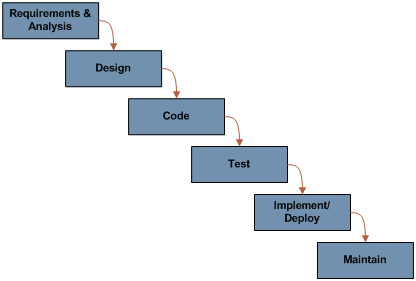
\includegraphics[width=100mm]{images/waterfall.png}
		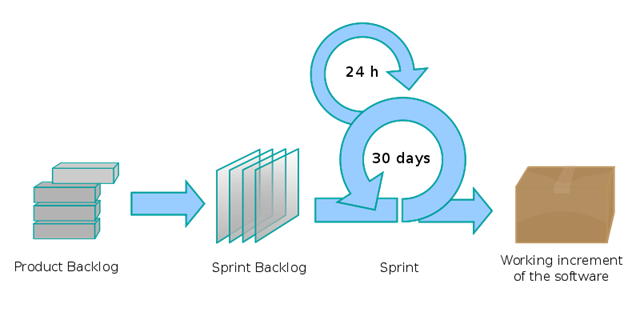
\includegraphics[width=100mm]{images/scrum.png}
		\caption{Software Lifecycles} 
		\label{lifecycles}
	\end{center}
\end{figure}

It has now been shown how to take algorithms, and parallelize them. How does this fit into developing software?
Although software must be built modularly from the beginning, actual parallelization should not occur until the 
end of the software development cycle. This comes from embraced design patterns in software engineering.
If code will take significant refactoring to make parallel, then it is incorrectly written from the beginning.

For example, in the code examples in this report, the function lapply is used. Major sections of code are organized in seperate functions. Changing the function from lapply to parLapply is almost all that is needed
to parallelize the code. 

In Figure \ref{lifecycles}, a few different software lifecycles are listed. \textbf{Waterfall} (top) is a good method if
the requirements for the project never change. Since this is seldom the case in research, Agile 
Development is encouraged. \textbf{Scrum} (bottom) contains many iterations of software development within
the project lifespan, in which a deliverable of the code is delivered. This allows the developers to react to 
changing requirements in the project, as well as a good way to gauge workflow in the project.

This report proposes a hybrid of this, in which there are several different phases of Scrums:

\begin{figure}[h]
	\begin{center}
		\includegraphics[width=160mm]{images/hybrid_scrum.png}
		\caption{Hybrid Scrum Project} 
		\label{hybrid_scrums}
	\end{center}
\end{figure}

The Development scrums start the project. It gives programmers a chance to learn the domain of the project, and try ideas that will be shape the project. This in when profiling of algorithms needs to occur, so reasonable 
data collection results. Implemenation scrums then create the main body of the code. The 
Optimization scrums come next. This is when existing code is streamlined. This phase is important, because it may eliminate the need for complicated parallelization. If granularities, or $P$ values, remain after this 
phase, then the Parallelization can take place.

\section{Conclusion}
In summary, this project showed even the author some suprising aspects of parallelism. In our own project,
the tail end of Amdahl's Law came much sooner than we thought. Applying parallel concepts can be difficult,
even for professionals. But it doesn't need to be. The concepts are simple in nature, and if good coding 
standards are accepted from the beginning, then the translation into parallel code will be easy.

The speedups that are seen in parallelism are very important. Without them, science of tomorrow will not be
possible. Researchers need to become familiar with the limitations of even parallel processing, and adjust their
project proposals accordingly. Not doing so will lead to failure. And a lack of understanding of parallelism may
cause a project to fail unnecessarily. HPC is the language of today, and we must all speak it to answer any 
questions about tomorrow.

%%%%%%%%% REFERENCES -- no limit

% this should include only items referenced in the project description
% it is not a bibliography of related reading.

% Each reference must include the names of all authors (in the same
% sequence in which they appear in the publication), the article and 
% journal title, book title, volume number, page numbers, and year of 
% publication. If the document is available electronically, the website 
% address also should be identified

\section{Bibliography}

\begin{thebibliography}{99}
\bibitem{mcgowan} Neptune, R.R.; McGowan, C.P. 
	"Muscle contributions to whole-body sagittal plane angular momentum during walking" 
	{ \em Journal of Biomechanics, 2011 }. 44 6–12 : Print.
\bibitem{amdahl} Amdahl, Gene (1967). "Validity of the Single Processor Approach to Achieving Large-Scale Computing Capabilities". {\em AFIPS Conference Proceedings} (30): 483–485. Print.
\bibitem{thelen} Thelen, D.G.; Anderson, F.C. "Using computed muscle control to generate forward dynamic simulations of human walking from experimental data"
	{ \em Journal of Biomechanics, 2006 }. 39 1107 - 1115: Print.
\bibitem{lloyd} Lloyd, G.L.; Besier, T. F.
	"An EMG-driven musculoskeletal model to estimate muscle forces and knee joint moments in vivo"
	{ \em  Journal of Biomechanics, 2003 }. 36 765-776: Print.
\end{thebibliography}

%\printglossaries



\end{document}
